\section{Gestione asset}
	Per quanto riguarda la gestione degli \mglo{Asset}{asset} l'utente ha la possibilità di:
	\begin{itemize}
		\item aggiungere un asset;
		\item visualizzare i dettagli relativi a un certo asset presente;
		\item modificare un asset presente;
		\item eliminare un asset presente.
	\end{itemize}

\subsection{Aggiunta di un asset}
	Per aggiungere un asset si deve:
	\begin{itemize}
		\item cliccare sul pulsante "+" in basso a destra della mappa;
		\item selezionare la voce "Aggiungi asset";
		\item disegnare il perimetro dell'asset sulla mappa. E' possibile apporre gli spigoli del perimetro cliccando direttamente sulla mappa. Il perimetro dell'asset deve essere correttamente chiuso, facendo coincidere l'ultimo spigolo del perimetro col primo;
		\item compilare i campi (tutti) rispettando i vincoli esposti nell'apposita appendice \nameref{Validazioni};
		\item cliccare sul pulsante "Salva", che verrà abilitato solo nel momento in cui tutte le operazioni sopra descritte sono state eseguite in maniera corretta.
	\end{itemize}
	
	\begin{figure}[H]
	\centering
	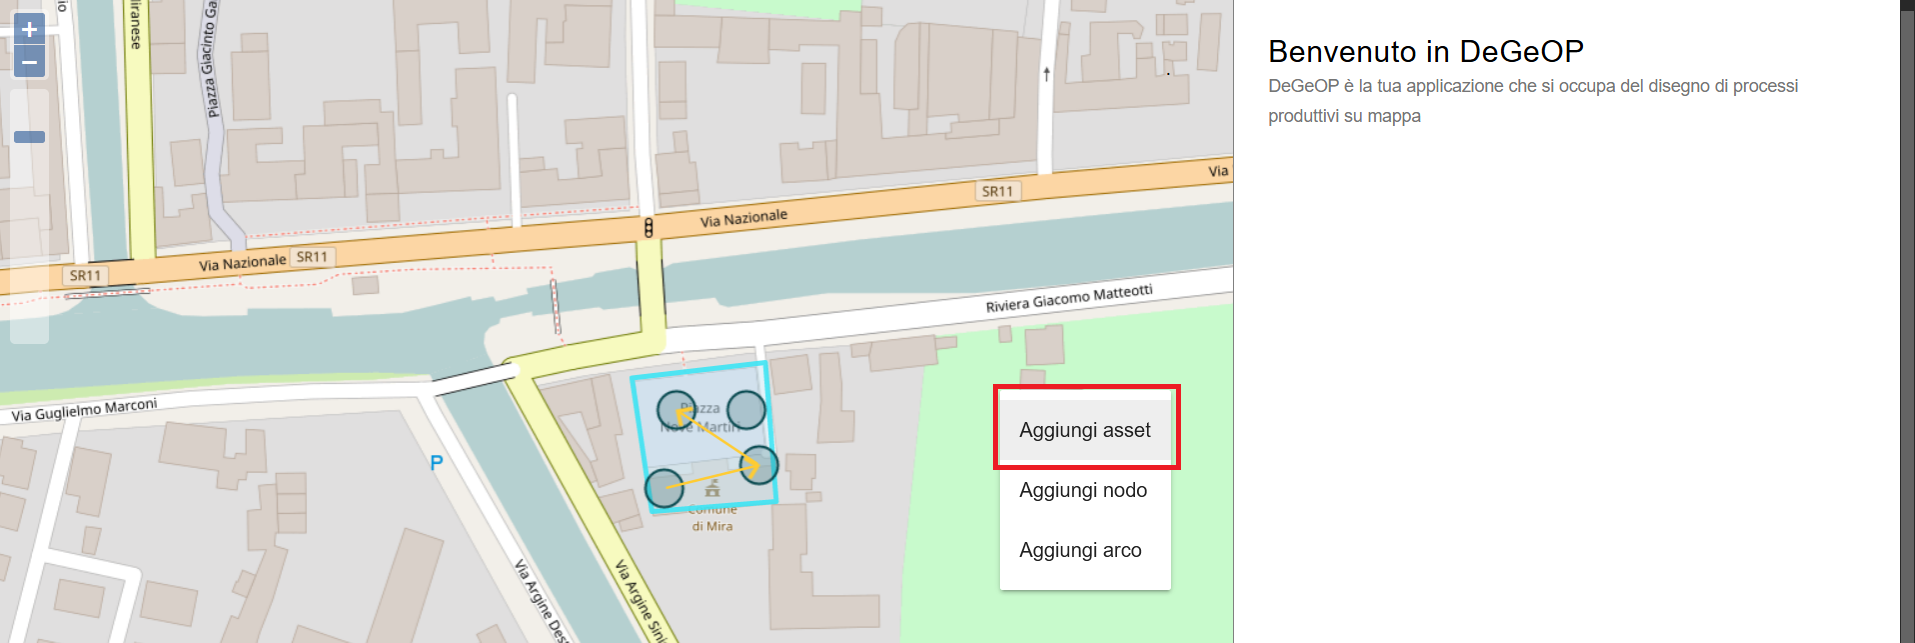
\includegraphics[width=\textwidth]{img/menu_aperto_asset_hover.png}
	\caption{Menu di aggiunta}
	\end{figure}
	
	\begin{figure}[H]
	\centering
	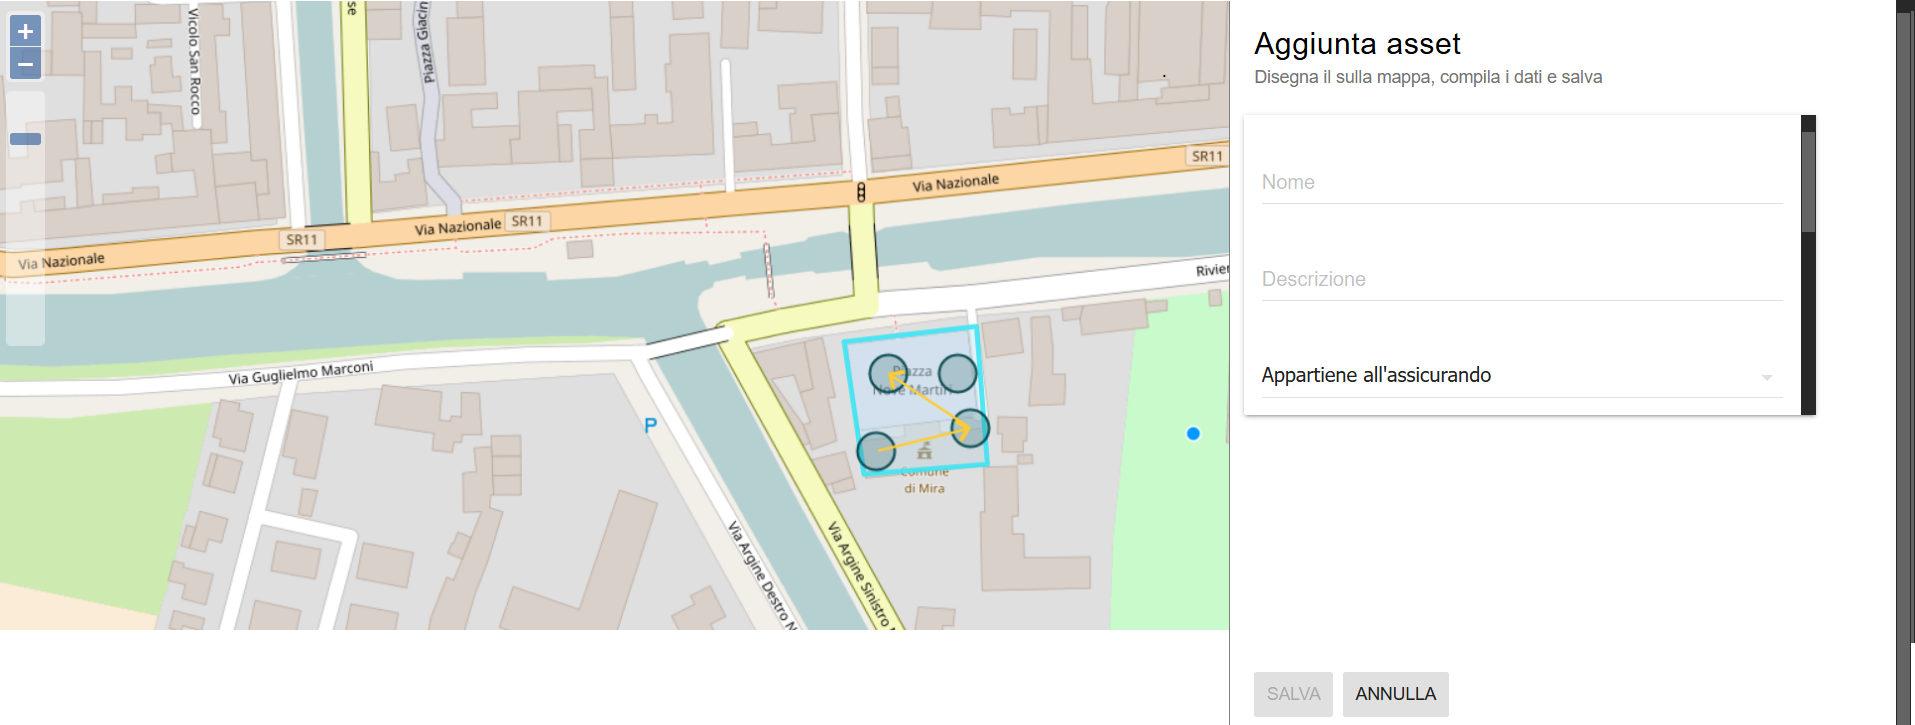
\includegraphics[width=\textwidth]{img/aggiunta_asset.png}
	\caption{Aggiunta di un asset}
	\end{figure}

\subsection{Visualizzazione dei dettagli di un asset}
	Per visualizzare i dettagli di un asset si deve:
	\begin{itemize}
		\item selezionare l'asset che si intende modificare cliccando direttamente su quell'asset dalla mappa.
	\end{itemize}
	
	\begin{figure}[H]
	\centering
	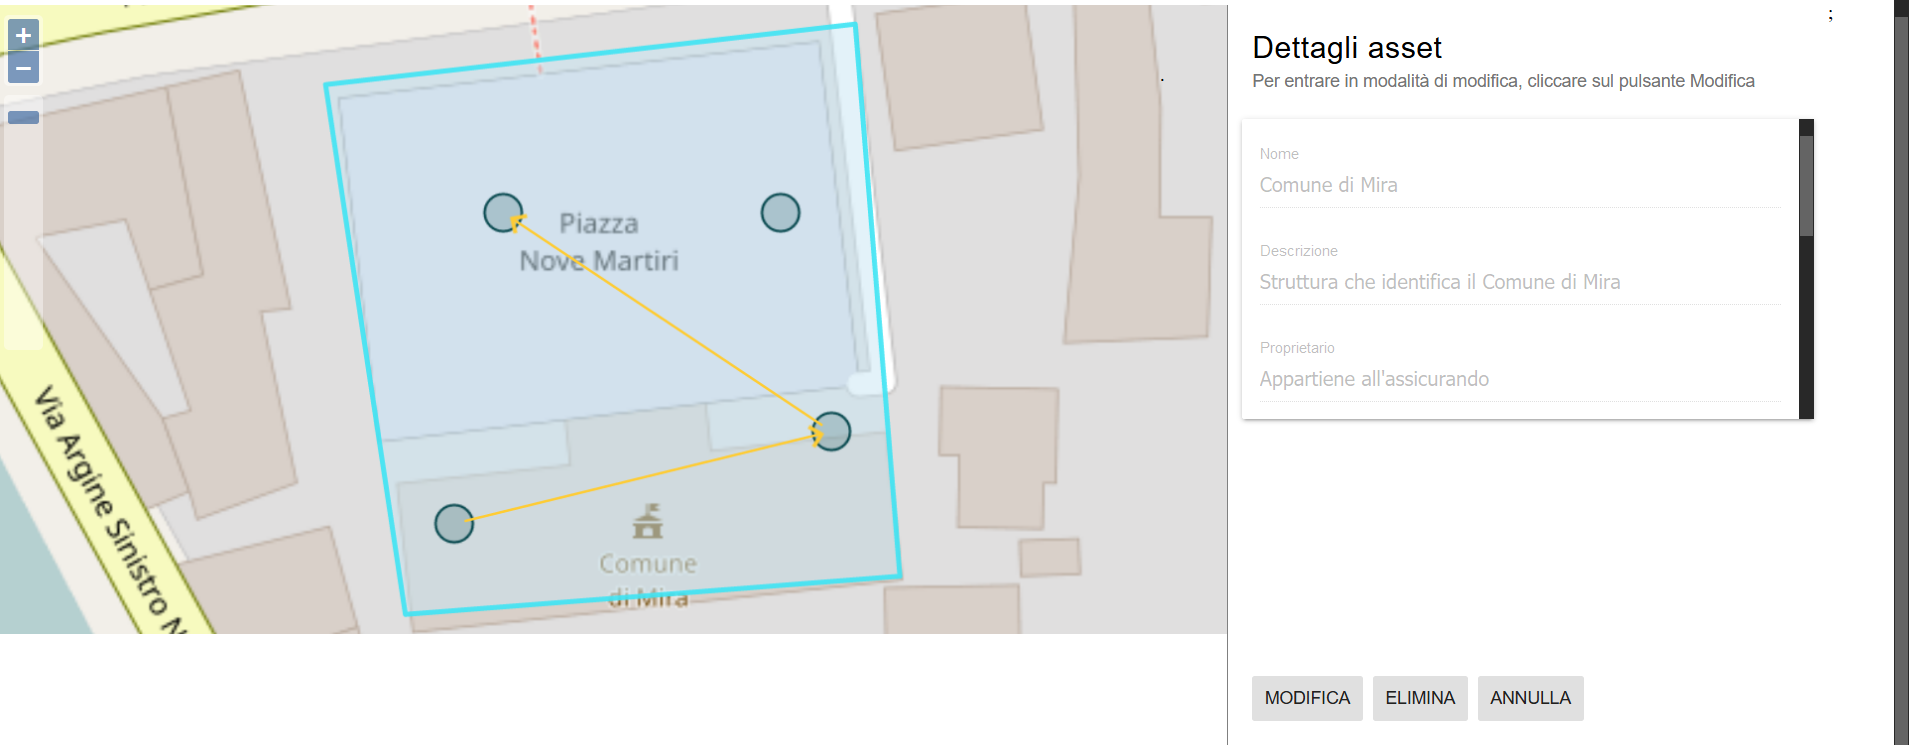
\includegraphics[width=\textwidth]{img/visualizzazione_asset.png}
	\caption{Visualizzazione dettagli di un asset}
	\end{figure}

\subsection{Modifica di un asset}
	Per modificare un asset si deve:
	\begin{itemize}
		\item selezionare l'asset che si intende modificare cliccando direttamente sulla mappa;
		\item cliccare sul pulsante "Modifica" in basso sulla sidebar;
		\item eventualmente ridisegnare il perimetro dell'asset sulla mappa. E' possibile apporre gli spigoli del perimetro cliccando direttamente sulla mappa. Il nuovo perimetro andrà in automatico a sovrascrivere quello precentemente presente. Il perimetro dell'asset deve essere correttamente chiuso, facendo coincidere l'ultimo spigolo del perimetro col primo;
		\item eventualmente modificare i campi rispettando i vincoli esposti nell'apposita appendice \nameref{Validazioni};
		\item cliccare sul pulsante "Salva", che verrà abilitato solo nel momento in cui tutte le operazioni sopra descritte sono state eseguite in maniera corretta.
	\end{itemize}
	
	\begin{figure}[H]
	\centering
	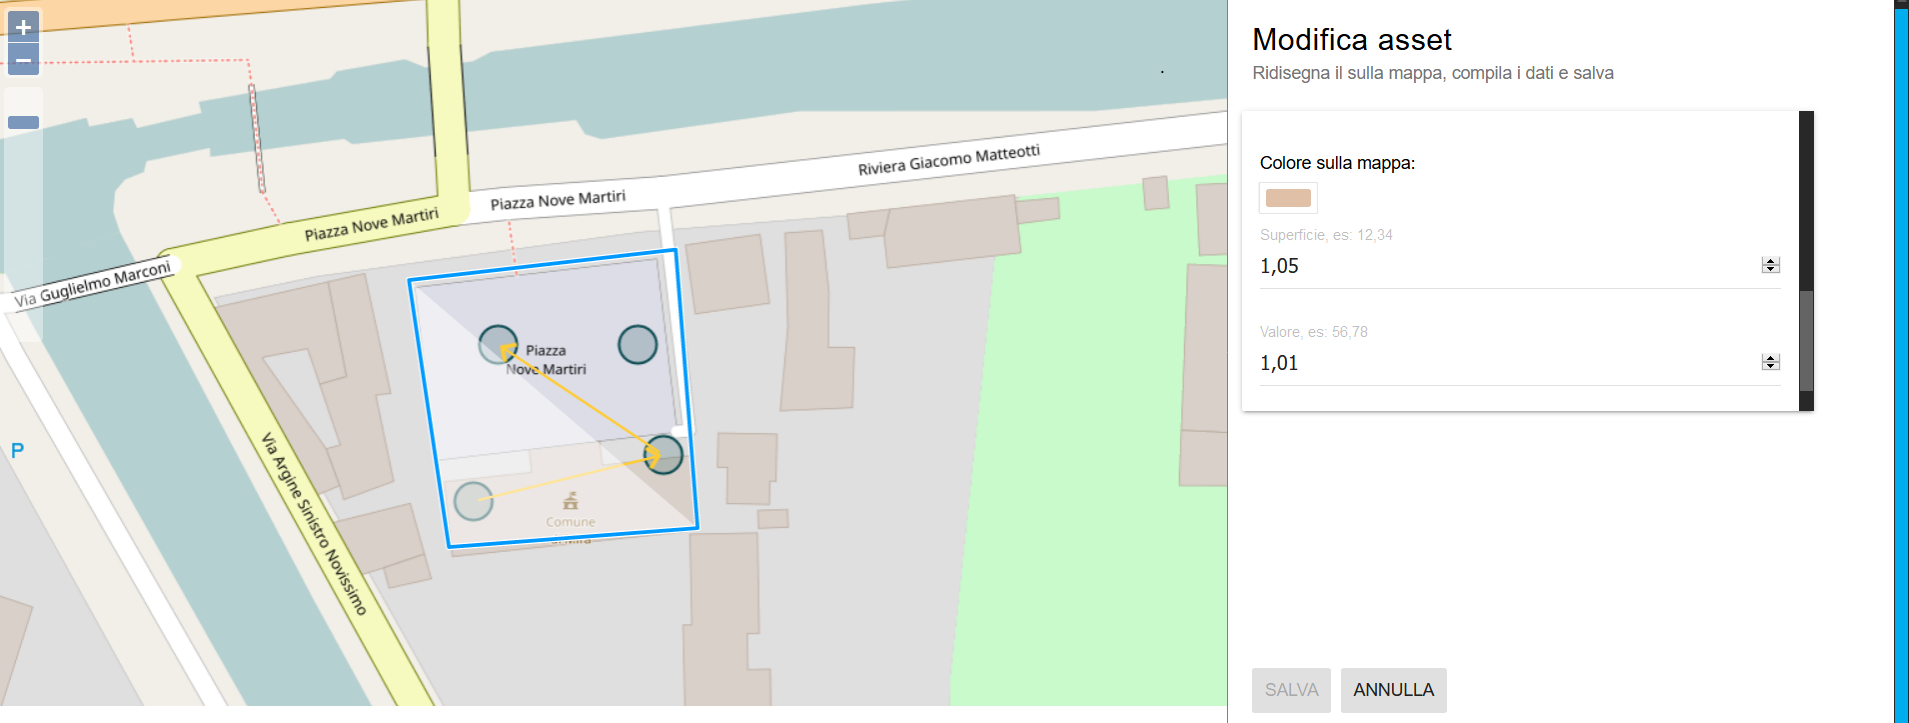
\includegraphics[width=\textwidth]{img/modifica_asset.png}
	\caption{Modifica di un asset}
	\end{figure}

\subsection{Eliminazione di un asset}
Si ricorda che eliminando un asset, verranno cancellati tutti i nodi in esso contenuti.
Per eliminare un asset si deve:
\begin{itemize}
	\item selezionare l'asset che si intende modificare cliccando direttamente sulla mappa;
	\item cliccare sul pulsante "Elimina" in basso sulla sidebar;
	\item cliccare sul pulsante "Elimina" sulla finestra bloccante che compare.
\end{itemize}

\begin{figure}[H]
\centering
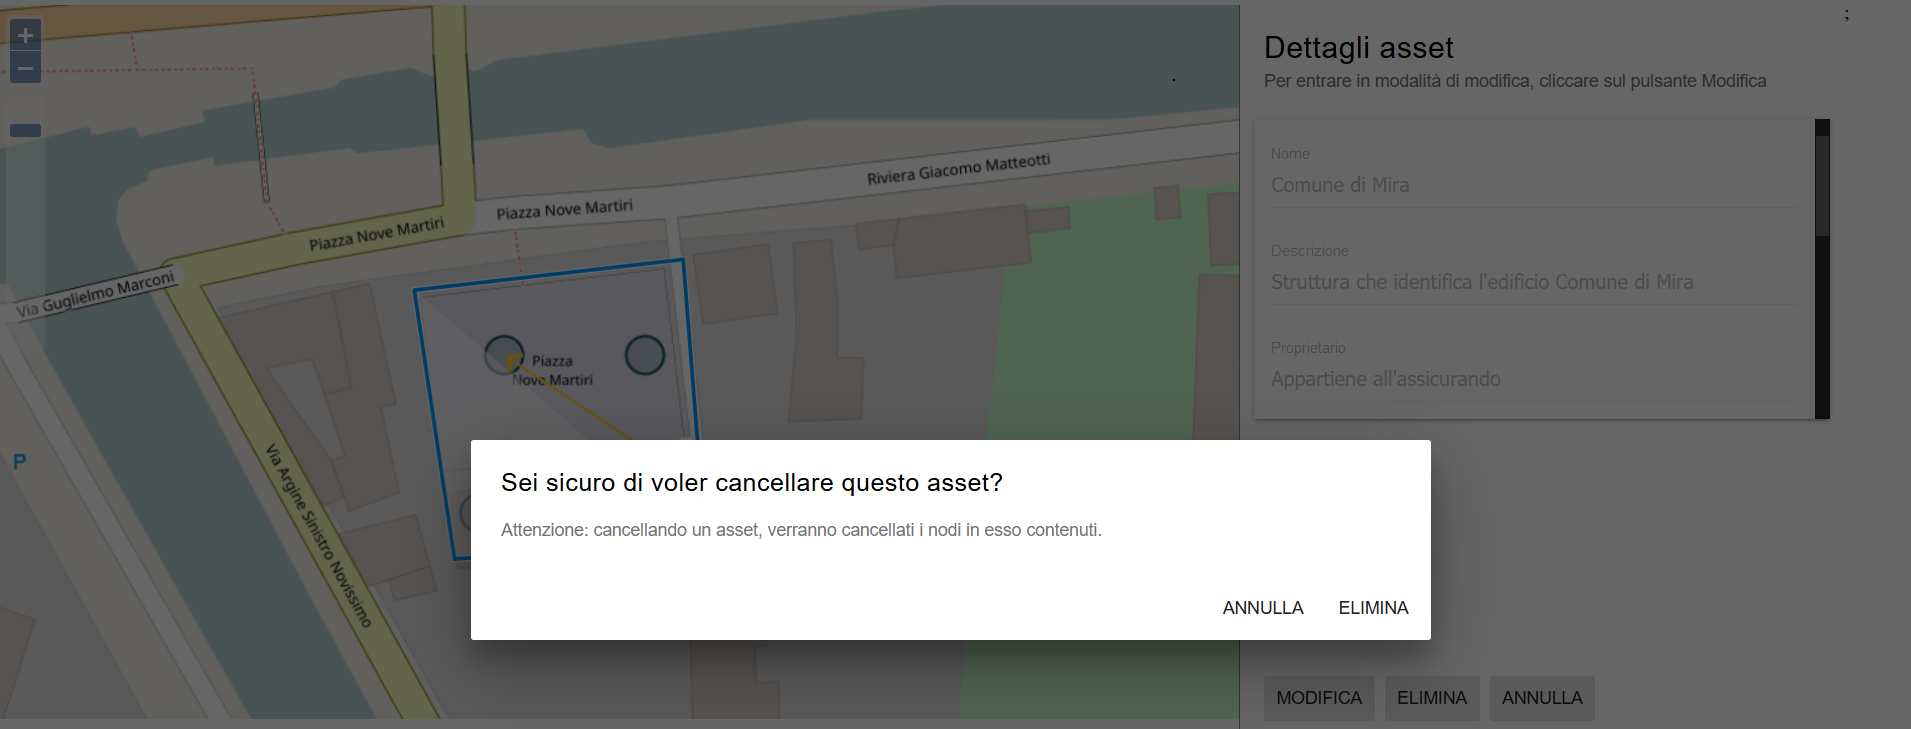
\includegraphics[width=\textwidth]{img/eliminazione_bloccante_asset.png}
\caption{Eliminazione di un asset}
\end{figure}